\documentclass{report}
\usepackage[utf8]{inputenc}
\usepackage{tikz}
\usetikzlibrary{shapes.geometric}
\usepackage{xcolor}
\usepackage{standalone}
\usepackage{amsmath}
\usepackage{amsfonts}
\usepackage{graphicx, color}
\usepackage[toc, page]{appendix}
\usepackage[a4paper,margin=3.5cm]{geometry}

\definecolor{h}{HTML}{228B22}
\definecolor{bias}{HTML}{87CEFA}
\definecolor{conv}{HTML}{FFA500}

\definecolor{bn}{HTML}{FFD700}
\tikzset{conv/.style={black,draw=black,fill=conv,rectangle,minimum height=1cm}}
\tikzset{bn/.style={black,draw=black,fill=bn,rectangle,minimum height=1cm}}
\tikzset{rcb/.style={draw, fill=bias, minimum height=1cm}}
\tikzset{elu/.style={draw, fill=h, minimum height=1cm}}

\newcommand{\red}[1]{{\color{red}{#1}}}

\newcommand{\bA}{\mathbf{A}}
\newcommand{\bB}{\mathbf{B}}
\newcommand{\bb}{\mathbf{b}}
\newcommand{\E}{\mathbb{E}}
\newcommand{\eye}{\mathbb{I}}
\newcommand{\Norm}{\mathcal{N}}
\newcommand{\Loss}{\mathcal{L}}
\newcommand{\bQ}{\mathbf{Q}}
\newcommand{\R}{\mathbb{R}}
\newcommand{\bR}{\mathbf{R}}
\newcommand{\bt}{\mathbf{t}}
\newcommand{\bU}{\mathbb{U}}
\newcommand{\bu}{\mathbf{u}}
\newcommand{\bw}{\mathbf{w}}
\newcommand{\bX}{\mathbf{X}}
\newcommand{\bx}{\mathbf{x}}
\newcommand{\by}{\mathbf{y}}
\newcommand{\bZ}{\mathbf{Z}}
\newcommand{\bz}{\mathbf{z}}

\newcommand{\eq}{=}
\newcommand{\parfrac}[2]{\frac{\partial #1}{\partial#2}}
\newcommand{\vectwo}[2]{\begin{pmatrix}#1\\#2\end{pmatrix}}
\newcommand{\vecthree}[3]{\begin{pmatrix}#1\\#2\\#3\end{pmatrix}}

\newcommand{\cneeded}{\footnote{Citation needed}}

\title{Causal Effect Inference using Normalizing Flows}
\author{Micha de Groot}


\begin{document}

%%%%%%%%%%%%%%%%%%%%%%%%%%%%%%%%%%%%%%%%%%%%%%%%%%%%%%%%%%%%%%%%%%%%%%%%%%%%%%%%
\begin{titlepage}

\newcommand{\HRule}{\rule{\linewidth}{0.5mm}} % Defines a new command for the horizontal lines, change thickness here
\center % Center everything on the page
 
%----------------------------------------------------------------------------------------
%	HEADING SECTIONS
%----------------------------------------------------------------------------------------


\includegraphics[width=\linewidth]{latex/Images/uvaENG.pdf}\\[2.5cm]
\textsc{\Large MSc Artificial Intelligence}\\[0.2cm]
% \textsc{\normalsize Track: \red{track}}\\[1.0cm] % track
\textsc{\Large Master Thesis}\\[0.5cm] 

%----------------------------------------------------------------------------------------
%	TITLE SECTION
%----------------------------------------------------------------------------------------

\HRule \\[0.4cm]
{ \huge \bfseries Causal Effect Inference\\ with Normalising Flows}\\[0.4cm] % Title of your document
\HRule \\[0.5cm]
 
%----------------------------------------------------------------------------------------
%	AUTHOR SECTION
%----------------------------------------------------------------------------------------

by\\[0.2cm]
\textsc{\Large Micha de Groot}\\[0.2cm] %you name
10434410\\[1cm]


%----------------------------------------------------------------------------------------
%	DATE SECTION
%----------------------------------------------------------------------------------------

{\Large \today}\\[1cm] % Date, change the \today to a set date if you want to be precise

48 EC\\ %
October 2019 - June 2020\\[1cm]%

%----------------------------------------------------------------------------------------
%	COMMITTEE SECTION
%----------------------------------------------------------------------------------------
\begin{minipage}[t]{0.4\textwidth}
\begin{flushleft} \large
\emph{Supervisor:} \\
Dr. Efstratios Gavves% Supervisor's Name
\end{flushleft}
\end{minipage}
~
\begin{minipage}[t]{0.4\textwidth}
\begin{flushright} \large
\emph{Assessor:} \\
\red{Dr A  \textsc{Person}}\\
\end{flushright}
\end{minipage}\\[2cm]

%----------------------------------------------------------------------------------------
%	LOGO SECTION
%----------------------------------------------------------------------------------------

%\framebox{\rule{0pt}{2.5cm}\rule{2.5cm}{0pt}}\\[0.5cm]
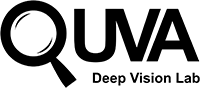
\includegraphics[width=2.5cm]{latex/Images/quva-logo-header.png}\\ % Include a department/university logo - this will require the graphicx package
\textsc{\large Instituut voor Informatica}\\[1.0cm] % 
 
%----------------------------------------------------------------------------------------

\vfill % Fill the rest of the page with whitespace

\end{titlepage}


\tableofcontents


%%%%%%%%%%%%%%%%%%%%%%%%%%%%%%%%%%%%%%%%%%%%%%%%%%%%%%%%%%%%%%%%%%%%%%%%%%%%%%%%
\chapter{Introduction}
Various scientific disciplines try to find patters in data. The patters that are usually uncovered are correlations between certain variables and features in the observations. In may fields this is a powerful tool that has resulted in tremendous scientific progress. Especially in AI we can perform a abundance of tasks by exploiting correlations in data, such as classification of images, translation of text or even the generation of new music \cite{deng2009imagenet} \cite{krizhevsky2012imagenet} \cite{bahdanau2014neural} \cite{payne2019musenet}.
But what a great deal scientists actually want to find out is what the causal relations of things are and correlations are merely a way to indicate a possible causal relation. The inherent problem with correlation-based methods is of course that the discovered correlations don't imply causation.

Every class in statistics starts with the phrase: "Correlation does not imply causation." This mantra tells us that we should never interpret a correlation between a variable $A$ and variable $B$ as '$A$ causes $B$'. This is very much true, but sometimes we do like to know: does $A$ cause $B$? To answer such questions we need causal inference. 

Causal inference is a process of quantifying causal relations between specific variables. This requires the isolation of causal effects between all related variables, which is not always possible if some of those variables are latent variables. Especially when we assume such a latent variable is a partial cause of both variables we are investigating, called latent confounding.

Disciplines such as medicine approach this problem through double-blind studies, in which the only difference between groups is whether or not they received a treatment, which eliminates any latent confounding. This means that any difference between the two trial groups must have been caused by the treatment\cite{gotzsche1989methodology}. Unfortunately the vast majority of problems can only be viewed through observational studies in which there usually is confounding between a variable $A$ and a variable $B$. Isolating the causal effect we are interested in from background variables in such cases can be a difficult task, as more than a century in statistical research has shown \cite{pearson1900x} \cite{fisher1936design} \cite{huff1993lie} \cite{ioannidis2005most}.

Fortunately the work by Pearl et al.\cite{pearl2009causal} \cite{pearl1995causal} has yielded a framework in which these causal effects can be modelled in terms of probability densities and in which it is theoretically possible to isolate a direct causal effect of a variable on another variable if there are one ore more unobserved confounding variables. This has led to a sub-field of scientific research within artificial intelligence on how to properly measure and analyse causal effects in the past two decades \cite{pearl2003statistics} \cite{hill2011bayesian} \cite{guo2020survey}\cite{mooij2016distinguishing}, especially focusing on how to leverage the ever-increasing amount of data that is available in artificial intelligence research.

In cases where there is latent confounding between the variables of interest, deep learning has a lot to offer, especially deep generative modelling. Deep generative modelling is of interest here because it can simultaneously learn a posterior distribution over the latent variables and learn the likelihood of the data. By modelling any latent confounding through a posterior over latent variables, we can correct for the effect of the latent confounding.  % We want to introduce the fact that we need a posterior over the confounders
Attempts at this have been done with the Causal VAE \cite{louizos2017causal} and to similar situations \cite{parafita2020causal}.  However, the VAE-based approach is limited in its expressiveness of the posterior distribution over the latent confounder. Parafita and Vitra \cite{parafita2020causal} show a promising direction for causal inference by suggesting the use of Normalising Flows, and therefore we will further investigate the use of generative modelling through the use of Normalising Flows \cite{rezende2016variational}. With this we hope to model the posterior distribution of the latent confounder more accurately, which can then be used to make more accurate predictions of any causal effect.

% Something about the shortcomings of other datasets and that/how we want to solve that. 
% This part is not clear
Earlier research in causal inference has relied mostly on semi-synthetic datasets, where part of the variables in the data were taken from a real empirical experiment and some of the variables were generated. The semi-synthetic setup still allows the experimenter to know the ground truth of certain parts in the causal process while keeping the experiment grounded in a real experiment. However, not knowing the ground truth of the entire process and its latent confounding disallows the experimenter to tweak specific components of the experimental setup. Furthermore, these datasets are limited in their complexity by the amount of variables that have been collected in the original observational studies, which potentially restrains a model in demonstrating its modelling power. 

Preliminary results on one such dataset, the Infant Health and Development Program (IHDP) dataset \cite{hill2011bayesian}, have shown that causal inference metrics on the dataset stagnate with more complex models, even though these models are able to achieve a better likelihood during optimisation. This could indicate that the complexity of the dataset used has been exhausted and the modelling power can only be seen in a more complex setting. That is why we propose a new completely synthetic dataset in this research, dubbed the Space Shapes dataset, to allow us to examine the influence of specific components in the dataset on the predictive power of the models that are used.

In this research we have two main research questions: Does the more flexible posterior of Normalising Flow-bases models allow us to make more accurate causal predictions than variational inference-based methods? And secondly: Does the increased complexity of the new Space Shapes dataset give insights on the modelling power of more complex models?

Our contributions are as follows:
\begin{itemize}
    \item A
    \item 
\end{itemize}
    % To what extent can the true direct causal effect between two variables be recovered from data when there is a latent confounder between the two variables, through the use of a proxy variable?
    
    % Does the more flexible posterior of Normalising Flow-bases models allow us to make more accurate causal predictions than variational inference-based methods?
    % \item Is the proposed causal flow model:
    
    %  - $<$better$>$ at estimating causal effects from data?
     
    %  - better at dealing with distributional shift in data?
     
    %  - capable of differentiating between distributions better 
     
    %  - More robust against latent confounding?
    % What does performance on the metrics that we use tell us?
    % Does it tell something only in comparison to the same metric in a different setting?
    % What aspect of the causal process is better learned by the flow-based model compared to the VAE-based model and other benchmarks?
    % How do certain types of normalising flows influence the predictive power of the causal flow?
    % In what way does the Space Shapes dataset give insights in the performance of causal inference models?



% The area of generative modelling within AI has shown a series of successes in recent years. This area tries to learn the structure within data and uncover the process with which it was generated. Such models have the power to <> the latent variables of the data. That ability is invaluable if we want to want to model latent confounders and be able to estimate causal effects. Using machine learning techniques also indicates that having mode data is useful for making more accurate predictions.


%In cases where it is not possible to directly use equation \ref{equation:do_operation}, we use a proxy variable $\bx$ instead. The work of Louizos et al. \cite{louizos2017causal} has show that this can to some extend be done by using VAEs \cite{kingma2013auto}. This approach had the problem that the variational lower bound did not become as high as theoretically possible. To circumvent that problem we propose an alternative approach by using Normalising Flows \cite{rezende2016variational} to model the posterior distribution of $\bZ$ and use that to calculate the Average Treatment Effect.



%%%%%%%%%%%%%%%%%%%%%%%%%%%%%%%%%%%%%%%%%%%%%%%%%%%%%%%%%%%%%%%%%%%%%%%%%%%%%%%%
% Dit hoofdstuk moet uitleggen wat het causality framework van Pearl is en vervolgens overgaan op ons soort probleem. Met een outcome, intervention, latent confounder en daarna de proxy. Hier komt ook dé causale graaf voor het eerst voor en introduceren we de belangrijkste notatie. Metrics komen hier ook naar voren, als we het hebben over de voorspelling die we willen doen. 
\chapter{Background and related work}
\section{Causal effect inference}
In the discipline of causal inference there are several questions that are commonly of interest. In this context we assume the framework of reasoning about causality as described by Pearl et al. \cite{pearl2009causal}, where relations between events are modelled as a Directed Acyclic Graph (DAG), and the state of each event is defined as a function of all its parents in said graph. What is interesting to know then are of course the structure of graphs and the form and parameters of each connection function. If the true graphs and functions would be know we would be able to precisely predict all causal effects. Of course such a bold claim follows by the observation that the search space of potential DAGs grows exponentially with the number of vertices, growing to $29281$ possible graphs when there are five vertices and $3781503$ possible graphs when then are six vertices \cite{robinson1977counting}. Some methods have been developed to address this problem, under some assumptions, but that goes beyond the scope of this research.

In this research we assume a given structure of the DAG and focus on finding the relation between the random variables in the graph. Specifically the effect of one variable, called the treatment and denoted with $\bt$, on one other variable, called the outcome and denoted with $\by$. % Move this

\subsection{Bayesian networks and Structural Causal Models}
Modelling various observed and unobserved variables in a DAG was originally proposed by Judea Pearl in the form of Bayesian networks \cite{pearl1985bayesian}. Although Bayesian networks can model conditional (in)dependencies through its edges, it can't model certain causal connections. A conditional probability of a variable $A$ on a variable $B$ can always be reversed but a causal connection can not.
This becomes relevant when we want to know the difference between observing variable $A$ and then variable $B$, and setting variable $A$ in a specific way and then observing variable $B$.

\subsection{Interventions and \textit{d}-separation}

\subsubsection{Notation}
Several variables will be used throughout this thesis, corresponding to nodes in the graphs in Figure \ref{fig:graph_observed_confounder_and_latent_with_proxy}. With $\bt$ and $\by$ we mean the variable that is the intervention and the variable on which we want to know the output effect, respectively. In short, the intervention variable $\bt$ and the outcome variable $\by$. Their latent confounder is indicated with $\bz$, and the proxy for the latent confounder with $\bx$.

\subsection{The \textit{do}-calculus and its use in causal inference}
The rules of \textit{do}-calculus allow us to quantify the causal effect of $\bt$ on $\by$ when there are one or more confounding variables, which is usually the case. This only requires the probability distributions and the structure of the causal graph defining the relation between all variables. As we assume the graph structure to be known we only need a correct factorisation of the joint distribution of all variables and we are practically done. An example is drawn in Figure \ref{fig:graph_observed_confounder_and_latent_with_proxy}. In this graph we can see what the confounding variables are that cause the two variables who's effect we want to measure, and correct for that by using the famous \textit{do}-operator equation:

\begin{figure}
    \centering
    \includestandalone{Figures/observed_confounder}
    \hspace{2cm}
    \includestandalone{Figures/causal_graph_one_proxy_one_confounder}
    \caption{Two causal Bayesian graphs, where all observed variables are coloured grey, unobserved variables are white and the causal relations are represented as arrows. The left hand side models an observed confounder and the right hand side a latent confounder with a proxy variable.}
    \label{fig:graph_observed_confounder_and_latent_with_proxy}
\end{figure}


\begin{equation}\label{equation:do_operation}
   p(\by | do(\bt)) = \int_{pa_\bt} p(\by | \bt, pa_{\bt}) p(pa_{\bt}) \text{d} pa_\bt
\end{equation}
The set $\text{pa}_\bt$ denotes the set of parent nodes from $\bt$ that satisfy the backdoor-criterion, which is only $\bZ$ in the case of left hand side graph in Figure \ref{fig:graph_observed_confounder_and_latent_with_proxy}. The problem is that in most real world scenarios we don't know what $\bZ$ is exactly and how these probabilities are shaped: it is a latent confounder. Most scientific disciplines that implicitly use this framework, such a double-blind medical trials, circumvent this problem by eliminating all possible latent confounders explicitly by making the cause of $\bt$ independent of everything else: a random assignment.

But in general this is not possible, and instead the principle of proxy variables is introduced\cneeded. These proxy variables, denoted with $\bX$, can be anything that can be measured and from which we can assume that it is directly caused by $\bZ$. The right hand side of Figure \ref{fig:graph_observed_confounder_and_latent_with_proxy} represent such a situation. The underlying principle of proxy variables is that it allows us to correct for the latent confounder in an approximate way. There has been extensive research in this area in recent years but most methods either assume that the latent confounder is categorical or 
% \cite{kuroki2014measurement} \cite{miao2018identifying}

\begin{equation}\label{equation:prediction_of_do_t}
    \begin{split}
        p(\by | \bx, do(\bt=t)) &= \int_{\bz} p(\by | \bx, do(\bt=t), \bz) p(\bz | \bx, do(\bt=t)) d\bz\\
        &= \int_{\bz} p(\by|\bt=t, \bz) p(\bz|\bx) d\bz
    \end{split}
\end{equation}

\subsection{Metrics in causal inference}
Precision in Estimation of Heterogeneous Effect(PEHE): $PEHE := \frac{1}{N}\sum\limits^N_{i=1}((y_{i1} - y_{i0}) - (\hat{y}_{i1} - \hat{y}_{i0}))^2$, where $y_1$ and $y_0$ correspond to the true outcomes under $t=1$ and $t=0$ respectively, and $\hat{y}_1$ and $\hat{y}_0$ correspond to the outcomes estimated by the model. 
Absolute error of the average treatment effect. Its the absolute error of the average of the individual treatment effect(ITE): 
\begin{equation}
    ITE(X) := \E[\by | \bX=x, do(\bt=1)] - \E[\by | \bX=x, do(\bt=0)], \quad ATE := \E[ITE(x)]
\end{equation}

we also have the CATE. I really don't understand what they are averaging over.
\begin{equation}
    CATE := \E[Y(1) - Y(0) | X=x] \quad Y(1) = \mu_1(X) + \epsilon(1) \quad Y(0) = \mu_0(X) + \epsilon(0)
\end{equation}


%%%%%%%%%%%%%%%%%%%%%%%%%%%%%%%%%%%%%%%%%%%%%%%%%%%%%%%%%%%%%%%%%%%%%%%%%%%%%%%%
% Hier introduceren we nog niks nieuws.
\section{Generative modelling and variational inference}
The field of variational inference is concerned with finding the posterior distribution of latent variables $\bz$ of some observed variables $\bx$. The purpose of this is to uncover the structure of the data distribution $p(\bx)$ and to make it possible to generate new samples from that distribution through the sampling of new $\bz$ from the prior\cite{bishop2006pattern}. The difficulty in this is that in general the posterior can have a complex structure and to uncover this requires us to solve an intractable integral:
\begin{equation}
    p_\theta(\bx) = \int p_\theta(\bx|\bz)p(\bz) d\bz
\end{equation}
A possible solution for this is the introduction of the variational distribution, $q_\phi(\bz|\bx)$ \cite{bishop2006pattern}. The variational distribution is an approximation for the real posterior that has a relatively simple form, for example a diagonal Gaussian. Through the introduction of the variational distribution we can derive a lower bound for the log-likelihood, called the evidence lower bound(ELBO) or negative free energy:

\begin{equation}\label{equation:negative_free_energy}
    \begin{split}
    \ln p_\theta(\bx) &= \ln \int p_\theta(\bx|\bz)p(\bz) d\bz\\
    &= \ln \int \frac{q_\phi(\bz|\bx)}{q_\phi(\bz|\bx)} p_\theta(\bx|\bz)p(\bz)d\bz\\
    &\geq \E_{q_\phi(\bz|\bx)}[\ln p_\theta(\bx|\bz) + \ln p(\bz) - \ln q_\phi(\bz|\bx)] \\
    &= D_{KL}[q_\phi(\bz|\bx) || p(\bz)] + \E_{q_\phi(\bz|\bx)}[\ln p_\theta(\bx|\bz)]= -\mathcal{F}(\bx)
    \end{split}
\end{equation}
This can be done quite effectively if both $p_\theta(\bx|\bz)$ and $q_\phi(\bz\bx)$ are modelled as neural networks. The work of \cite{kingma2013auto} has show how to then optimise this lower bound through stochastic gradient descent(SGD) methods, through the use of the reparameterisation trick. Such a model is called the Variational Autoencoder(VAE). It is capable of constructing a meaningful latent representation of data and to generate new data samples from that latent space. 

A weakness of the VAE is that the learned variational distribution can't be too complex, even if the true posterior would be. Another disadvantage is the difficulty of finding the global optimum of the model when using a non-linear neural network. Furthermore, the work of \cite{alemi2017fixing} has shown that even if a good marginal log-likelihood is obtained, the model may still have learned a weak latent representation.

\subsection{Normalising Flows}
The research in generative models has yielded a model type called Normalising Flows, first thought of by Tabak and Turner \cite{tabak2013family} and later popularised by Rezende and Mohamed \cite{rezende2016variational}. The approach of this class of models is to learn a series of invertible mappings from a simple prior distribution to the distribution of the data, which is assumed to be far more complex. This is done through the change of variable equation \ref{equation:change_of_variables}. Through this equation, it is guaranteed that before and after the transformations we have a valid probability distribution, and with the use of the inverse of these mappings, one can perform exact posterior inference. 


\begin{equation}\label{equation:change_of_variables}
    \bx = f(\bz) \qquad p(\bx) = p(\bz) \left|\text{det} \parfrac{f}{\bz} \right|^{-1}
\end{equation}
The reason we talk about a series of transformations is to split the the potentially complex mapping in Equation \ref{equation:change_of_variables} into smaller, simpler transformations. This results then in Equation \ref{equation:change_of_variables_log_chain}, given in log-space, as is conventional. Here we have $K$ functions $f_k$ mapping from latent variables $\bz_{k-1}$ to $\bz_k$ and ending with the mapping from $\bz_{K-1}$ to $\bx$.

\begin{equation}\label{equation:change_of_variables_log_chain}
    \ln p(\bx) = \ln p(\bz_0) - \sum\limits^K_{k=1}\ln \left| \text{det} \parfrac{f_k}{\bz_{k-1}} \right|
\end{equation}
To make this work in practice the (log)determinant of the Jacobian of each mapping $f_k$ has to computed efficiently. The most straightforward way to do this is to enforce that each mapping has a triangular Jacobian. This immediately solves the second practical criterion of having a tractable inverse of each $f_k$. Another more implicit requirement for our mappings is that they are parameterised functions on which we can use gradient descent methods to learn the parameters. 

The original paper that introduced the Normalising Flow had a slightly different approach. Instead of mapping from the data distribution to the latent prior or the other way around, it maps the latent variable to its more expressive final posterior. This approach extends the idea of a VAE with a Normalising Flow. In the first part of the inference procedure a data sample $\bx$ is mapped to the parameters of the (simple) variational distribution. In the second step the first latent variable in the flow, $\bz_0$ is sampled from this distribution, and in the third step $\bz_0$ is mapped through the Normalising Flow to the final posterior estimate $\bz_K$. By rewriting the negative free energy function we get the following lower bound of the log-likelihood:

\begin{equation}\label{equation:negative_free_energy_with_flow}
    \begin{split}
    -\mathcal{F}(\bx) &= -D_{KL}[q_\phi(\bz|\bx) || p(\bz)] + \E_{q_\phi(\bz|\bx)}[\ln p_\theta(\bx|\bz)]\\
    &= \E_{q_\phi(\bz|\bx)}[-\ln q_\phi(\bz|\bx) + \ln p(\bz) + \ln p_\theta(\bx|\bz)]\\
    &= \E_{q_0(z_0)}[-\ln q_0(\bz_K) + \ln p(\bz) + \ln p_\theta(\bx|\bz_K)]\\
    &= \E_{q_0(z_0)}[-\ln q_0(\bz_0) + \sum\limits^K_{k=1}\ln \left|\text{det} \parfrac{f_k}{\bz_{k-1}} \right| + \ln p(\bz) + \ln p_\theta(\bx|\bz_K)]\\
    \end{split}
\end{equation}
where we have $q_0(z_0)$ as the start of the flow, while also being a variational distribution. Several implementations of Normalising Flows have been made so far, some of which we will discuss here briefly.

\subsubsection{Planar flow and radial flow}\label{section:planar_radial_flow}
In the original work of Rezende and Mohamed \cite{rezende2016variational}, two possible implementations were proposed. The first one is the planar flow, in which each mapping has the form:
\begin{equation}\label{equation:planar_flow}
    f(\bz) = \bz + \bu h(\bw^T\bz + b)
\end{equation}
where $\bw \in \R^D$, $\bu \in \R^D$ and $b \in \R$ are learnable parameters and $h(\cdot)$ is a smooth element-wise non-linearity with derivative $h'(\cdot)$. The determinant of the Jacobian of such a transformation is defined as:
\begin{equation}\label{equation:planar_flow_logdet}
    \det\parfrac{f(\bz)}{\bz}  = 1 + \bu^T h'(\bw^T \bz + b)\bw
\end{equation}
Each transformation here can be seen as a layer in a neural network that consists of a skip connection and a single-node dense layer followed by an expansion back to the original number of dimensions. The downside of this is the limited transformative capabilities of each mapping in the flow, which means that in practice a long sequence of such functions is needed to reach a complex posterior.

The second implementation proposal of Rezende and Mohamed is the radial flow. This family of transformations applies radial contractions and expansions around a reference point $\bz_0$:
\begin{equation}
    f(\bz) = \bz + \beta h(\alpha, r)(\bz - \bz_0)
\end{equation}
where $r$ and $h$ are defined as $r=|\bz - \bz_0|,  h(\alpha, r) = 1/(\alpha + r)$, and $\bz_0 \in \R^D$, $\alpha \in \R^+$, $\beta \in \R$ are learnable parameters. This also has a Jacobian determinant that can be computed in linear time, having the following log-likelihood:
\begin{equation}
    \det \parfrac{f(\bz)}{\bz}  = (1 + \beta h(\alpha, r))^{D-1} (1 + \beta h(\alpha, r) + \beta h'(\alpha, r)r)
\end{equation}
with $h'(\cdot)$ the derivative of $h(\cdot)$ Both the planar flow and the radial flow have restrictions on their learnable parameters to ensure that the transformations are invertible, but these pose no further limitations on the transformative capabilities in practice.

\subsubsection{Sylvester flow}
As mentioned in the previous section, the planar flow acts as a skip connection with a single-node dense layer. The Sylvester Normalising Flow\cite{berg2018sylvester} solves the limitation of this bottleneck by allowing a higher dimensional transformation:
\begin{equation}\label{equation:sylvester_flow_A_B}
    f(\bz) = \bz + \bA h(\bB\bz + \bb)
\end{equation}
where $\bA \in \R^{D\times M}$, $\bB \in \R^{M\times D}$ and $\bb \in \R^M$ are learnable parameters and $h(\cdot)$ is again a smooth element-wise non-linearity. The scalar value $M \leq D$ is a hyperparameter that determines the bottleneck dimensions. We note the planar flow is now a special case of the Sylvester flow when $M=1$. The determinant of the Jacobian in this form cannot be computed in linear time, as it requires the calculation of the determinant of a full matrix, nor is this transformation invertible in general:
\begin{equation}\label{equation:sylvester_logdet}
    \det \parfrac{f(\bz)}{\bz} = \det (\eye_M + \text{diag}(h'(\bB\bz + \bb))\bB\bA)
\end{equation}
To solve both problems, van den Berg et al. propose a special case of equation \ref{equation:sylvester_flow_A_B}, where $\bA$ and $\bB$ are QR-factorised:
\begin{equation}\label{equation:sylvester_flow_Q_R}
    f(\bz) = \bz + \bQ\bR h(\widetilde{\bR}\bQ^T\bz + \bb)
\end{equation}
where $\bR$ and $\widetilde{\bR}$ are upper triangular $M \times M$ matrices and $\bQ$ is an orthogonal $D \times M$ matrix. Combining equation \ref{equation:sylvester_logdet} and \ref{equation:sylvester_flow_Q_R} yields the following Jacobian determinant:
\begin{equation}
        \det \parfrac{f(\bz)}{\bz} = \det (\eye_M + \text{diag}(h'(\widetilde{\bR}\bQ^T\bz + \bb))\widetilde{\bR}\bR)
\end{equation}
This can again be computed in linear time and has the guarantee that $f(\bz)$ is invertible if $\bR$ and $\widetilde{\bR}$ are invertible. 


\subsubsection{Real-valued Non-Volume Preserving transformations}
As mentioned at the start of the chapter, Normalising Flows can also be used to directly learn a mapping from the data distribution to a prior, which directly optimises the data log-likelihood instead of the ELBO. A type of Normalising Flow that does this is the Real-valued Non-Volume Preserving transformation (real NVP) \cite{dinh2016density}. By using so-called coupling layers, this model type encompasses all affine Normalising Flows. Each transformation in this model consists of two coupling layers, where each coupling layers transforms one half of the current variable vector $\bz_k \in \R^D$ and keeps the other half fixed, done in the following way:
\begin{align}\label{equation:real_nvp_coupling}
    \bz_{k+1, 1:d} &= \bz_{k, 1:d} \\
    \bz_{k+1, d+1:D} &= \bz_{k, d+1:D} \odot \exp \left(s(\bz_{k, 1:d}) \right) + t(\bz_{k, 1:d})
\end{align}
where $s$ and $t$ are scale and translation functions respectively, $\R^{d} \rightarrow \R^{D-d}$. By having one coupling layer transforming $\bz_{d+1:D}$ and the next layer transforming $\bz_{1:d}$ the whole variable is transformed. The Jacobian of one coupling layer is triangular:
\begin{equation}
    \parfrac{\bz_{k+1}}{\bz_k^T} = \begin{bmatrix}
    \eye_d & 0\\
    \parfrac{\bz_{k+1, d+1:D}}{\bz_{k, 1:d}^T} & \text{diag}(\exp(s(\bz_{k, 1:d}))
    \end{bmatrix}
\end{equation}
which gives an easy to compute log determinant: $\sum\limits^d_{i=1} s(\bz_{k, 1:d})_i$. The log-determinant Jacobian  does not require us to compute a Jacobian or determinant of either $s$ or $t$. Computing the inverse of each coupling layer doesn't require the inverse of $s$ or $t$ either, as we only need to invert the multiplication and addition:
\begin{align}\label{equation:real_nvp_coupling_inverse}
    \bz_{k, 1:d} &= \bz_{k+1, 1:d} \\
    \bz_{k, d+1:D} &= (\bz_{k+1, d+1:D} - t(\bz_{k+1, 1:d})) \odot \exp \left(- s(\bz_{k+1, 1:d}) \right) 
\end{align}
The simplicity of these equations allow us to choose $s$ and $t$ arbitrarily complex, by choosing a deep neural network for example. The split of each vector $\bz_k$ into two halves can be done arbitrarily, not requiring the elements of the two halves to be consecutive elements. The pattern in from which the two halves are constructed have a variety op options. The authors of \cite{dinh2016density} suggest to  either use a checkerboard pattern, if the data consists of images, or to reshape the input to contain a multiple of the original number of channels and alternate between channels to which half of the split they belong. In all cases is is pertinent to transform values every other coupling layer.

\subsubsection{Nonlinear Squared Flows}
The transformation in equation \ref{equation:real_nvp_coupling} is an affine transformation. Although this can result in complex transformations, if enough coupling layers are used, a single affine coupling is still restricted. A more flexible variation of the affine coupling has been proposed by \cite{ziegler2019latent}, called the nonlinear squared flow. This flow type changes the coupling function to a non-linear version by adding an additional term to it:
\begin{align}\label{equation:nonlinear_squared_flow}
    \bz_{k+1, 1:d} &= \bz_{k, 1:d} \\
    \bz_{k+1, d+1:D} &= \bz_{k, d+1:D} \odot \exp (a)  + b + \frac{c}{1 + (\bz_{k, d+1:D} \odot \exp (d) + g)^2}
\end{align}
where $a, b, c, d, g$ are all functions of $\bz_{k, 1:d}$, $\R^{d} \rightarrow \R^{D-d}$. The inversion of this transformation is a bit more complex and requires the root of a cubic polynomial. Therefore the parameters are constrained to a certain extend. However, the advantage of this coupling function is that even in the one dimensional case it is able to transform a unimodal distribution to a multimodal distribution.

%%%%%%%%%%%%%%%%%%%%%%%%%%%%%%%%%%%%%%%%%%%%%%%%%%%%%%%%%%%%%%%%%%%%%%%%%%%%%%%%
% Hier bespreken we:
%  - CEVAE
%  - CEVAE + PF
%  - Het idee van context
%  - Het idee van elk ding zijn eigen prior geven
%  - Samen brengen naar het laatse model
\chapter{Causal effect inference with generative models}
The idea of using a generative model in causal effect inference was proposed by Louizos et al. \cite{louizos2017causal}. They leveraged the power of VAEs to make it possible to infer latent confounders from data without any prior knowledge on the confounder itself.

\begin{figure}
    \centering
    \includestandalone[width=0.59\textwidth]{Figures/cevae_encoder_figure}
    \caption{Graph of the encoder of the Causal VAE. Nodes in white are neural networks and nodes in grey are sampling steps or data input. The $q(\bt|\bx)$ and $q(\by|\bt, \bx)$ are input nodes of the network during training but the values of $\bt$ and $\by$ are sampled during test time.}
    \label{fig:cevae_encoder_graph}
\end{figure}
\begin{figure}
    \centering
    \includestandalone[width=0.45\textwidth]{Figures/cevae_decoder_figure}
    \caption{Graph of the decoder of the causal VAE. Nodes in white are neural networks and nodes in grey are sampling steps.} 
    \label{fig:cevae_decoder_graph}
\end{figure}

The objective function of a CEVAE is of the same form as the ELBO in equation  \ref{equation:negative_free_energy}. It is the expectation under the variational distribution of the joint log probability of all variables, minus the log of the variational distribution:
\begin{equation}
    \mathcal{L} = \E_{q_\phi(\bz|\bx, \bt, \by)}[\ln p_\theta(\bx, \bt | \bz) + \ln p_\theta(\by |\bt, \bz) +\ln p(\bz) - q_\phi(\bz | \bx, \bt, \by)]
\end{equation}

\section{Causal effect inference with Normalising Flows}
This can be potentially be improved upon by using Normalising Flows. Their ability to reproduce the true posterior over the latent confounder is an improvement on the CEVAE. The first proposal for this is to pass the inferred $\bZ$ values through a series of Normalising Flows to yield $\bZ_k$, which can then be used to reconstruct the observed variables. We can implement this the simplest by using Planar Flows, as described in section \ref{section:planar_radial_flow}. Through this we hope to uncover a better match to the true posterior of $\bZ$.

\noindent
New definition of the ELBO:
\begin{equation}
    -\mathcal{F}(\bx) = \mathbb{E}_{q_0(\bz_0)}\left[\ln p(\bx, \bt | \bz_K) + \ln p(\bz) + \ln p(\by |\bt, \bz_K) - \ln q_0(\bz_0) + \sum\limits^K_{k=1} \ln \left| 1 + \bu_k^Th'(\bw^T_k\bz_{k-1} + b)\right| \right]
\end{equation}


% Deze moet helemaal opnieuw getekend worden
\begin{figure}
    \centering
    \includestandalone{Figures/cenf_with_vae}
    \caption{Visualisation of the Causal VAE, augmented with a normalising flow. The encoder part on the left is the same as in Figure \ref{fig:cevae_encoder_graph} and the decoder on the right is the same as in Figure \ref{fig:cevae_decoder_graph}. The flow in the middle can be any type of normalising flow.}
    \label{fig:cenf_with_vae}
\end{figure}

\subsection{Augmenting decoder with a Normalising Flow}
A possible way to extend this approach is to model $p(\bt|\bt,\bz)$ with a flow as well. In the original model there are two MLPs that model both $p(\by|\bt=1,\bz)$ and $p(\by|\bt=0,\bz)$. If we want our model to be able to generalise to more complex interventions we need to step away from an approach that requires multiple networks for multiple values of $\bt$. The problem that we face then is that the distribution of $p(\by|\bt,\bz)$ might not be a simple diagonal Gaussian. That is where Normalising Flows come into play. They might be able to capture the more complex distribution. 

The immediate problem that we face is that in the simpler datasets $\by$ is just 1-dimensional. This means that we would have a flow that is also 1-dimensional, which might require a very long flow to make it work.

\begin{equation}
    \ln p(\by_K|\bt, \bz) := \ln p(\by_0|\bt, \bz) - \sum\limits^K_{k=1} \ln \left | \parfrac{g_k}{\by_{k-1}} \right|
\end{equation}



\subsection{Causal Flow}
The augmentation to the causal VAE described in the previous section allows the model to learn a more complex posterior of the data, but the general structure is the same; the model is still optimising a lower bound of the likelihood and is still limited to modelling the observed variables with parameterised distributions. To alleviate these limitations we propose the causal flow. This model splits Equation \ref{equation:prediction_of_do_t} in two parts, similar to the causal VAE, as can be seen in Figure \ref{fig:causal_flow_with_y_prior}. One part of the model, estimates the value of $\bz$ for a given $\bx$. The second part of the model does the intervention and predicts the outcome value. Both of these halves are modelled by a normalising flow:
\begin{equation}
    \bx = f(\bz), \qquad \ln p(\bx) = \ln p(\bz) - \sum \ln \left|\det \parfrac{f(\bz)}{\bz}\right| 
\end{equation}
where the function $f$ can be any function that satisfies the criteria for a normalising flow. We optimise this by passing each data point through the inverse of the flow $f^{-1}$ and maximising its likelihood. For the second half we add a new variable to the graph: a prior over $\by$, and we make use of 'context' in a normalising flow \cite{papamakarios2019normalizing} \cite{dinh2016density}. The 'context' of a normalising flow is an additional input to the mapping. It can't be part of either of the two random variables at either end of the mapping. A second constraint is that the 'context' cannot be part of the Jacobian, % something something inverse
This allows us to model a conditional distribution, such as the one we need here:
\begin{equation}
    \by = g(\by_{prior}, \bt, \bz), \qquad \ln p(\by) = \ln p(\by_{prior}) - \sum \ln \left|\det \parfrac{g(\by_{prior}, \bt, \bz)}{\bz}\right| 
\end{equation}

\begin{figure}
    \centering
    \includestandalone[width=0.45\textwidth]{Figures/causal_flow_with_y_prior_training}
    \qquad
    \includestandalone[width=0.45\textwidth]{Figures/causal_flow_with_y_prior_testing}
    \caption{Causal flow model. The model on the left hand side indicates the direction of the flows during training and the model on the right hand side indicates the direction of the flow during testing. Full lines indicate a Normalising Flow between two variables, a dashed line indicates that a variable is used as a context variable in the flow.}
    \label{fig:causal_flow_with_y_prior}
\end{figure}


% Hier moet de rest van mijn model contribution worden uitgelegd. Het causal VAE gedeelte moet duidelijk hebben dat het eerder werk is. En dan twee secties of wat ik heb toegevoegd. Eentje met de causal VAE+planar flow en eentje met causal flow. Dan hernoem ik H4 naar iets anders. Model misschien? Of causal inference using normalising flows.

%%%%%%%%%%%%%%%%%%%%%%%%%%%%%%%%%%%%%%%%%%%%%%%%%%%%%%%%%%%%%%%%%%%%%%%%%%%%%%%%
\chapter{Experiments}

\section{Experimental setup}
% Hier iets over de metrics?
% Tensorflow noemen ergens
Wat in ieder geval? Uiltleg dat we een nn trainen voor x epochs en met welke hyperparameters allemaal. Wat hebben we nog meer qua experiment setup? Het doel uiteindelijk is factual en counterfactual voorspellingen doen voor de outcome variable. Moet ik hier de DAG noemen die we gebruiken of is het logischer om dat eerder te doen? Het is eerder een onderdeel van de experimental setup. Dan moet hoofdstuk twee algemener blijven en nog niet in gaan op specifieke instanties van een DAG.

\section{Ablations or something?}

\section{Datasets}
We will perform experiments on three datasets. The first dataset has been a widely used dataset to benchmark causal effect inference. The second dataset was proposed by \cite{louizos2017causal} for the causal VAE experiments, and the third dataset is a new dataset we propose for causal effect inference research. Each dataset consists of a set of triplets, where each triplet contains the proxy variable, the factual intervention variable and the factual outcome variable.

\subsection{Infant Health and Development Program}
The Infant Health and Development Program(IHDP) dataset is a semi-synthetic dataset that was proposed by \cite{hill2011bayesian}. This dataset is based on a randomised controlled trial testing the efficacy of early intervention to enhance the cognitive, behavioural, and health status of low birth weight, premature infants \cite{ramey1992infant}. 

From this original dataset \cite{hill2011bayesian} selected a nonrandom subset to dis-balance the intervention and the outcome, and took the measured covariates of the mothers as proxy variable. This resulted in a dataset of 747 samples with 25-dimensional proxy variables and a binary intervention variable. The outcome variables were simulated, based on these original variables. This allowed a potentially larger dataset by repeating the simulation process multiple times.

\subsection{Twin Births}
The second dataset is also a semi-synthetic dataset. It is based on a medical trial on the effect of birth weight on infant mortality\cite{almond2005costs}. The randomisation was in this original experiment achieved by only researching twins and the intervention being that one of the twins was born heavier than the other. This results in always having both a factual and counterfactual case, if the assumption that twins are similar enough holds. Fortunately the real outcome of child mortality if very low ($3,5\%$ first year mortality). Therefore \cite{louizos2017causal} et al. made the decision to select only those twins where both weighted less than $2kg$, yielding a dataset of 11984 twins.

\subsection{Space Shapes}
Lastly we propose a new dataset ourselves. This dataset is a completely synthetic dataset, which has images as a proxy variable instead of a regular feature vector. Each proxy variable consist of a 60 by 60 pixels RGB image which shows six simple shapes, each with a different colour. The intervention variable is a 2-dimensional vector that dictates the steering or movement of the red circle in each image. The outcome variable is the relative distance form the red circle's new position to the centre right of the image. See Figure \ref{fig:space_shapes_sample} for a visualisation of this. 

If we would keep the setup as described up to now, there would be no latent confounding, since the outcome could be directly calculated, given the position of the red circle in the image and the value of the intervention vector. This would reduce most of the prediction task to detecting the red circle in the image and make inference of the latent variables redundant. Therefore we added latent confounding in the following way. Each other shape in the image is assigned a 'gravity' value that is constant for that shape-colour combination throughout the dataset. This gravity influences the position of the red circle during the intervention by an amount relative to the distance between the red circle and the other shapes. This entails that the position of the red circle would change even when the intervention would be zero. More details on the exact data generation can be read in Appendix \ref{}.

\begin{figure}
    \centering
    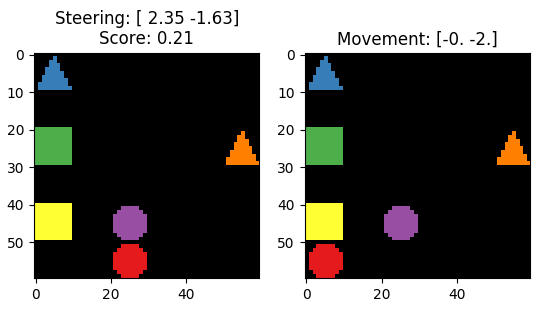
\includegraphics{latex/Images/sample_space_shapes_score_left.png}
    \caption{Sample of the Space Shapes dataset, with the observed variables on the right. The 2-dimensional steering vector is the intervention variable, the score scalar is the outcome variable and the image is the proxy variable. The image on the right is a visualisation of the process that underlies the outcome variable. The 2-dimensional vector is the combined effect of the intervention variable and the latent confounding 
   'gravity' effects.}
    \label{fig:space_shapes_sample}
\end{figure}

The data is inspired on the datasets used by \cite{kipf2019contrastive} and \cite{kumar2019videoflow}, who both propose their own image dataset with moving shapes. The research of \cite{kipf2019contrastive} looks at this from a reinforcement learning perspective, where the image is an initial state and the intervention is considered an action. The goal is also to learn the result of the action but the dataset by Kipf et al. does not contain any latent confounding between the states and actions. The VideoFlow model by Kumar et al. has similar images, but instead of one image and one interventions takes a series of images as input and has as task to predict a (short) sequence of images that could continue the sequence.


%%%%%%%%%%%%%%%%%%%%%%%%%%%%%%%%%%%%%%%%%%%%%%%%%%%%%%%%%%%%%%%%%%%%%%%%%%%%%%%%
\chapter{Results}

\renewcommand{\arraystretch}{1.3}
\begin{table}[]
    \centering
    \begin{adjustbox}{center}
    \begin{tabular}{l||c|c|c||c|c|c||c|c|c|}
        %  & & IHDP & & & TWINS & & & SPACE &\\
        & \multicolumn{3}{|c||}{IHDP} & \multicolumn{3}{|c||}{TWINS} & \multicolumn{3}{|c|}{SPACE} \\ 
         Model & ATE & ITE & PEHE & ATE & ITE & PEHE & ATE & ITE & PEHE \\
         \hline \hline
         TARNET & $\mathbf{2.24\text{e-}}1$ & $1.490$ & 2.126 &   $8.3\text{e-}2$ & $6.51\text{e-}1$ & $3.50\text{e-}1$ &     $6.96\text{e-}1$ & 2.191 & 1.241\\
         \hline
         CEVAE & $4.18\text{e-}1$ & 1.443 & 2.497 &    $1.09\text{e-}1$ & $\mathbf{3.84\textbf{e-}1}$ & $3.29\text{e-}1$ & $5.43\text{e-}1$ & 1.917 & $6.74\text{e-}1$\\
         \hline
         CEVAE + PF & $4.75\text{e-}1$ & $\mathbf{1.379}$ &  2.662 & $1.22\text{e-}1$ & $\mathbf{3.83\text{\text{e-}}1}$ & $3.27\text{e-}1$ & $6.84\text{e-}1$ & 1.913 & $5.55\text{e-}1$ \\
         \hline
         CEVAE + RF & . & . & . &  . & . & . & $3.256\text{e-}1$ & $1.978$ & $3.98\text{e-}1$\\
         \hline 
         CEVAE + SF & . & . & . &  . & . & . & $1.189\text{e-}1$ & $1.915$ & $1.486\text{e-}1$\\
         \hline
         NCF: affine & $3.32\text{e-}1$ & $1.796$ & $\mathbf{1.995}$ &    $\mathbf{3.00\text{e-}2}$ & $6.85\text{e-}1$ & $\mathbf{3.16\text{e-}1}$ & \textbf{$\mathbf{5.03\text{e-}2}$} & $\mathbf{1.846}$ & \textbf{$\mathbf{5.15\text{e-}2}$} \\
         \hline
         NCF: nonlinear & . & . & . & $5.91\text{e-}2$ & $6.72\text{e-}1$ & $3.20\text{e-1}$\\
    \end{tabular}
    \end{adjustbox}
    \caption{The scores of each model on each dataset. The cell in bold indicates the best score in each column. The scores on the SPACE dataset here are the scores on the same version as the models were trained on.}
    \label{tab:results_experiments}
\end{table}

\begin{table}[]
    \centering
    \begin{adjustbox}{center}
    \begin{tabular}{l||c|c|c||c|c|c||c|c|c|}
        %  & & IHDP & & & TWINS & & & SPACE &\\
        & \multicolumn{3}{|c||}{More objects} & \multicolumn{3}{|c||}{tbd} & \multicolumn{3}{|c|}{tbd} \\ 
        Model & ATE & ITE & PEHE & ATE & ITE & PEHE & ATE & ITE & PEHE \\
        \hline \hline
        TARNET &  \\
        \hline
        CEVAE & \\
        \hline
        CEVAE + PF & \\
        \hline
        CEVAE + RF & \\
        \hline 
        CEVAE + SF & \\
        \hline
        NCF: affine & \\
        \hline
        NCF: nonlinear & \\
    \end{tabular}
    \end{adjustbox}
    \caption{The scores of each model on variations of the SPACE dataset. Each model was trained on the original version of the dataset and tested on a version with one alteration. The cell in bold indicates the best score in each column}
    \label{tab:results_experiments_space}
\end{table}


%%%%%%%%%%%%%%%%%%%%%%%%%%%%%%%%%%%%%%%%%%%%%%%%%%%%%%%%%%%%%%%%%%%%%%%%%%%%%%%%
\chapter{Discussion and conclusion}


%%%%%%%%%%%%%%%%%%%%%%%%%%%%%%%%%%%%%%%%%%%%%%%%%%%%%%%%%%%%%%%%%%%%%%%%%%%%%%%%
\bibliography{references.bib}
\bibliographystyle{apalike}


\begin{appendices}
\chapter*{Generation process of the SPACE dataset}
The SPACE dataset is generated in several steps. Setting up all prior information, generating initial states, interventions and outcome states, and converting the used representation to images. For the first step the following hyperparameters are needed. All of these can be changed manually to create a slightly different dataset:
\begin{enumerate}
    \item Height and width of the scene as whole number. These two numbers determine the size of the grind in which the objects are placed. Their product cannot be lower than the total number of objects.
    \item Number of different colours and number of different shapes the objects can take. It is recommended that these two numbers are coprime as to allow the most actually different looking objects.
    \item Total number of different objects that can exist. This can at most be the number of colours times the number of shapes, if those two numbers are coprime. Otherwise the maximum has to be divided by their common divisors.
    \item Colour scale factor and shape scale factor. These two factors determine the difference in scaling the prior of the gravity differs between object of a different colour and objects of a different shapes respectively.
    \item The 'prior' dimensions. This dimensionality determines the 
\end{enumerate}

...

Gravity per object
\begin{align}
    colour factor_c &= \left(1 + \frac{c * colour scale factor}{\# colours} \right)\\
    shape factor_s &= \left(1 + \frac{s * shape scale factor}{\#shapes}\right) \\
    gravity factor_n &= colour factor_n * shape factor_n \\
    gravity_n &\sim \Norm(gravity factor_n, 1)
\end{align}

Then we sample from the intervention prior and the positions prior:
\begin{align}
    I_M &\sim \Norm(0, I)\\
    P_M &\sim \Norm(0, I)\\
    prior &\sim \Norm(0, I)\\
    Prior &= \begin{pmatrix}gravity_1 \\ \vdots\\gravity_N \\ prior\end{pmatrix}\\
\end{align}

Next we use these priors to compute the weights of the distribution that governs the positions of the objects in the initial states and sample these positions:
\begin{align}
position_n \sim Mult(\sigma(Prior \cdot P_M)_n, 1)    
\end{align}

Then we calculate the move of the 'space ship':
\begin{align}
    distance_n &= position_n - position_0\\
    direction &= P \cdot I_m +\sum\limits^N_{n=1} distance_n * gravity_n\\
    new position &= position_0 + direction
\end{align}

\chapter*{Architecture of networks used}
Most models described in this paper use several neural networks as components of the larger model. Their exact architectures are described here.

\section*{Convolutional networks}
Each network that has images as input uses the same convolutional network architecture, as can be seen in Figure \ref{fig:conv_net}. This consists of blocks with a batch normalisation, exponential linear unit and convolutional layer. Furthermore, the model has several skip connections between each set of three blocks.

\section*{Fully connected networks}
All other neural networks take (abstract) feature vectors as input. These networks are set up as fully connected networks with exponential linear units as nonlinearities.

\begin{figure}
    \centering
    \includestandalone[]{Figures/conv_res_net}
    \hspace{1cm}
    \includestandalone[]{Figures/conv_block}
    \caption{Convolutional residual network that is used on the left. The Block components are shown in full on the right.}
    \label{fig:conv_net}
\end{figure}


\end{appendices}
\end{document}